\newpage
\section {Билет 25. Модели логического разграничения доступа: мандатная, дискреционная, ролевая. Атрибутивная модель.}

\begin{center}
	\textit{\underline{Политика разграничения доступа}}
\end{center}

\textbf{Политика разграничения доступа} - набор правил, определяющий условия, при которых допускается выполнение той или иной операции над данными, т.е. отвечает на следующие вопросы: <<Кому? Что? И для каких данных можно сделать?>>\\

\textbf{Разграничение доступа} - техники реализации политики информационной безопасности. Существует два класса разграничения доступа:
\begin{itemize}
 \item \textbf{Физическое разграничение} - ограничение физического доступа к данным: закрытие помещений, изоляция устройств и т.д.
 \item \textbf{Логическое разграничение} - ограничение на уровне сущностей информационной системы (файлов, записей в БД, сетевого доступа).
\end{itemize}

Далее рассмотрим различные модели \textbf{логического разграничения}. Здесь тоже можно выделить два класса моделей:
\begin{enumerate}
	\item Проверка условий доступа ВО ВРЕМЯ выполнения конкретных операций над данными. 
	\item Проверка условий доступа ДО выполнения конкретных операций над данными.
\end{enumerate}

\textbf{Первый тип} проверок условий доступа может выполняться прямо в коде операции и например выглядеть следующим образом:
\begin{algorithm}
\begin{algorithmic}[H!]
	\If{(Условия доступа НЕ выполнены)}
	\State *Ошибка*
	\EndIf
	
	\State *Выполняем операцию*
\end{algorithmic}
\end{algorithm}


Данные проверки можно также реализовать за счет разных конструкций присущих разным языкам (Декораторы, Метаклассы - Python; Mixin'ы, Наследования - С++; и т.д). Также опишем достоинства и недостатки данного подхода.

\begin{figure}[H]
	\centering
	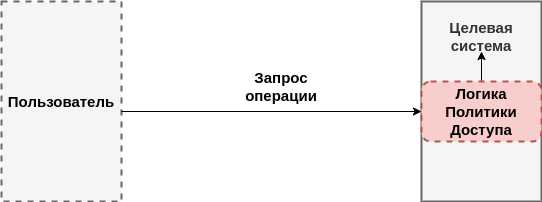
\includegraphics[scale = 0.7]{25/AC_in.png}
	\caption{Логика доступа внутри операции}
	\label{fig:ac_in}
\end{figure}


\begin{itemize}
	\item \textbf{Достоинства}:
	\begin{enumerate}
		\item Гибкость, так как можно производить любые вычисления и реализовывать сложную логику.
	\end{enumerate}
	\item \textbf{Недостатки}:
	\begin{enumerate}
		\item Логика политики распределена по исходному коду. Соответственно для ее изменения нужно менять значительную часть исходного кода операции.
		\item Невозможно анализировать <<корректность>> реализованной политики, так как она реализована на алгоритмически полном языке (или Тьюринг полном языке) то данная задача сводиться к нерешенной \href{https://clck.ru/pui5M}{<<проблеме остановки>>}. В связи с чем высока вероятность ошибки, которую очень сложно выявить.
	\end{enumerate}
\end{itemize}


\textbf{Второй тип} проверок условий доступа выделяет логику доступа в отдельную <<сущность>> и дает возможность реализовать ее на не алгоритмически полном языке.
\begin{itemize}
	\item \textbf{Достоинства}:
	\begin{enumerate}
		\item Вся логика содержится в одном месте и для ее изменения нужно менять малую часть кода.
		\item Из-за алгоритмической (Тьюринг) не полноты возможен анализ и верификация логики, в связи с чем количество сложно выявляемых ошибок стремиться к нулю.
	\end{enumerate}
	\item \textbf{Недостатки}:
	\begin{enumerate}
		\item Из-за алгоритмической (Тьюринг) не полноты возможно не получится реализовать все возможные варианты логики политики доступа.
	\end{enumerate}
\end{itemize}

\begin{figure}[H]
	\centering
	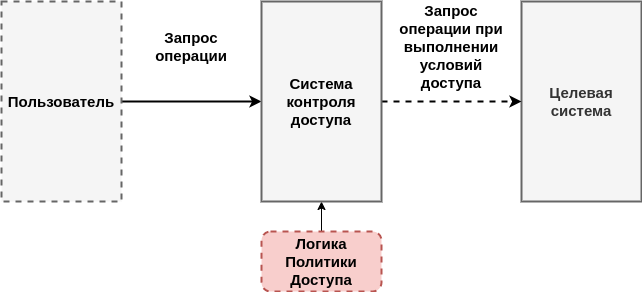
\includegraphics[scale = 0.7]{25/AC_out.png}
	\caption{Логика доступа вне операции}
	\label{fig:ac_out}
\end{figure}

На практике используются большое количество различных моделей политик разграничения доступа (DAC, MAC, RBAC, HBAC, IBAC, CBAC, ABAC, GBAC, ...). Рассмотрим несколько наиболее распространенных.

\begin{center}
	\textit{\underline{Мандатная (MAC)}}
\end{center}

\textbf{Мандатная, MAC(Mandatory Access Control)} - Принудительный контроль доступа. В модели \textbf{MAC} каждому объекту назначается метка конфиденциальности (Не секретно, для служебного пользования, секретно, совершенно секретно, и т.д.), а пользователю выдаются допуски. Данная модель используется в ядре ОС Linux и во многих других ОС к которым предъявляются высокие требования к безопастности, изменение меток как правило производится только администраторами. 

В данной модели на метках конфиденциальности и допусках пользователя вводится отношение порядка, например: $$\text{Не секретно} < \text {Для служебного пользования} < \text{Секретно} < \text {Совершенно секретно}$$

Причем должны выполняться следующие условия:
\begin{itemize}
	\item Пусть дана метка $m_i$, тогда для любых $m_j > m_i$ пользователь с допуском $m_i$ не имеет права ни на какие операции для данных с метками $m_j$.
	\item Пусть дана метка $m_i$, тогда для любых $m_j < m_i$ пользователь с допуском $m_i$ имеет право только на <<чтение>> данных с меткой $m_j$.
\end{itemize}

Из недостатков можно выделить невозможность предоставление доступа только к части данных в рамках одной метки, например нельзя дать доступ только к одной части документов с метками <<Совершенно секретно>> для пользователей с соответствующим доступом.

\begin{center}
	\textit{\underline{Дискреционная (DAC)}}
\end{center}

\textbf{Дискреционная, DAC(Discretionary Access Control)} - Избирательный контроль доступа. В модели \textbf{DAC} доступ к объекту осуществляется на основе матрицы доступа (например по столбцам все данные, а по строчкам все пользователи и в пересечении нужных строк и столбцов стоит метка обозначающая какой доступ разрешен/запрещен) или на основе списков управления доступом (список пользователей имеющих доступ к данным). Для каждой пары (субъект(пользователь) — объект(данные)) должно быть задано явное и недвусмысленное перечисление допустимых типов доступа (читать, писать и т. д.), то есть тех типов доступа, которые являются санкционированными для данного субъекта (индивида или группы индивидов) к данному ресурсу (объекту).

Возможны несколько подходов к построению дискреционного управления доступом:
\begin{itemize}
\item Каждый объект системы имеет привязанного к нему субъекта, называемого владельцем. Именно владелец устанавливает права доступа к объекту.
\item Система имеет одного выделенного субъекта — суперпользователя, который имеет право устанавливать права владения для всех остальных субъектов системы.
\item Субъект с определённым правом доступа может передать это право любому другому субъекту.
\end{itemize}

Возможны и смешанные варианты построения, когда одновременно в системе присутствуют как владельцы, устанавливающие права доступа к своим объектам, так и суперпользователь, имеющий возможность изменения прав для любого объекта и/или изменения его владельца. Именно такой смешанный вариант реализован в большинстве операционных систем, например Unix или Windows NT.

\begin{center}
	\textit{\underline{Ролевая (RBAC)}}
\end{center}

\textbf{Ролевая, RBAC (Role Based Access Control)} - Ролевой контроль доступа. Модель \textbf{RBAC} является развитием политики избирательного управления доступом (DAC), при этом права доступа субъектов системы на объекты группируются с учётом специфики их применения, образуя роли (Директор, Секретарь, Бухгалтер и т.д. ).

Формирование ролей призвано определить чёткие и понятные для пользователей компьютерной системы правила разграничения доступа. Ролевое разграничение доступа позволяет реализовать гибкие, изменяющиеся динамически в процессе функционирования компьютерной системы.

Такое разграничение доступа является составляющей многих современных компьютерных систем. Как правило, данный подход применяется в системах защиты СУБД, а отдельные элементы реализуются в сетевых операционных системах. Ролевой подход часто используется в системах, для пользователей которых чётко определён круг их должностных полномочий и обязанностей.

Так как привилегии не назначаются пользователям непосредственно и приобретаются ими только через свою роль (или роли), управление индивидуальными правами пользователя по сути сводится к назначению ему ролей. Это упрощает такие операции, как добавление пользователя или смена подразделения пользователем.

Для определения модели RBAC используются следующие соглашения:
\begin{itemize}
\item $S$ = Субъект = Человек или автоматизированный агент (множество пользователей);
\item $R$ = Роль  = Рабочая функция или название, которое определяется на уровне авторизации (множество ролей);
\item $P$ = Разрешения = Утверждения режима доступа к ресурсу (множество прав доступа на объекты системы);
\item $SE$ = Сессия = Соответствие между S, R и/или P
\item $SA$ = Назначение субъекта
\item $PA: R \to 2^p$ — функция, определяющая для каждой роли множество прав доступа; при этом для каждого $p \in P$ существует $r \in R$ такая, что $p \in PA(r)$;
\item $RH$ = Частично упорядоченная иерархия ролей. $RH$ может быть еще записана так: ≥
\item Один субъект может иметь несколько ролей.
\item Одну роль могут иметь несколько субъектов.
\item Одна роль может иметь несколько разрешений.
\item Одно разрешение может принадлежать нескольким ролям.
\end{itemize}


Роли назначаются субъектам, вследствие чего субъекты получают те или иные разрешения через роли. RBAC требует именно такого назначения, а не прямого назначения разрешений субъектам, иначе это приводит к сложно контролируемым отношениям между субъектами и разрешениям. На возможность наследования разрешений от противоположных ролей накладывается ограничительная норма, которая позволяет достичь надлежащего разделения режимов. Например, одному и тому же лицу может быть не позволено создать учётную запись для кого-то, а затем авторизоваться под этой учётной записью.

Используя нотацию теории множеств, $x ≥ y$ означает, что $x$ наследует разрешения $y$:
\begin{itemize}
\item $PA \subseteq P \times R$, при этом разрешения назначаются связям ролей в отношении «многие ко многим».
\item $SA \subseteq S \times R$, при этом субъекты назначаются связям ролей и субъектов в отношении «многие ко многим».
\item $RH \subseteq R \times R$
\end{itemize}

\begin{center}
	\textit{\underline{Атрибутивная (ABAC)}}
\end{center}

\textbf{Атрибутная, ABAC (Attribute Based Access Control)} - Атрибутный контроль доступа. Модель \textbf{ABAC} является развитием политики избирательного управления доступом (DAC) и политики ролевого контроля доступа. Рассматриваемый вид разграничения доступа даёт возможность создать огромное количество комбинаций условий для выражения различных политик. Например дать доступ Бухгалтеру на запись некоторых данных только в промежутке между 9 и 18 часов.


